\section{Lektion 20-03-2018}

\begin{enumerate}
	\item DSP Run-Time Library
	\item Cycles Measurement
	\item Complex Numbers
	\item Filter IIR, FIR- FFT, iFFT
	\item Convolution
	\item Statistical (Auto+Cross-correlation)
\end{enumerate}

\subsection{DSP Run-Time Library}
\begin{itemize}
	\item Integer Arithmetic to Encode Fractional Semantic
	\begin{itemize}
		\item Not supported by Run-Time Lib
	\end{itemize}
	\item  Built-In Functions (compiler intrinsics)
	\begin{itemize}
		\item \mintinline{cpp}{fract16, fract32}
		\item Fully supported by Run-Time Lib
	\end{itemize}
	\item Native Fixed-Point Types (fract and accum)
	\begin{itemize}
		\item \mintinline{cpp}{fract, long fract, accum}
		\item Partly supported by Run-Time Lib
	\end{itemize} 
\end{itemize}

\subsubsection{Conversions}
\begin{itemize}
	\item The \mintinline{cpp}{stdflx.h} provides functions to conversions
	\item Useful for converting between native types (\mintinline{cpp}{fract}, \mintinline{cpp}{long fract}) and integer typedefs (\mintinline{cpp}{fract16}, \mintinline{cpp}{fract32}). 
	\item Convert a bit pattern to a fixed-point type \mintinline{cpp}{bitsfx} \item Convert a fixed-point type to a bit pattern \mintinline{cpp}{fxbits}
	\item \mintinline{cpp}{[hr, r, lr, uhr, ur, or ulr]}
	\item Conversion float to fract/fract16
	\begin{itemize}
		\item \mintinline{cpp}{fract16 af16 = float_to_fr16(a);}
		\item \mintinline{cpp}{a = fr16_to_float(af16);}
	\end{itemize} 
\end{itemize}

\subsubsection{Fixed-Point Type Constant Suffixes and Macros}
\begin{figure} [H]
	\centering
	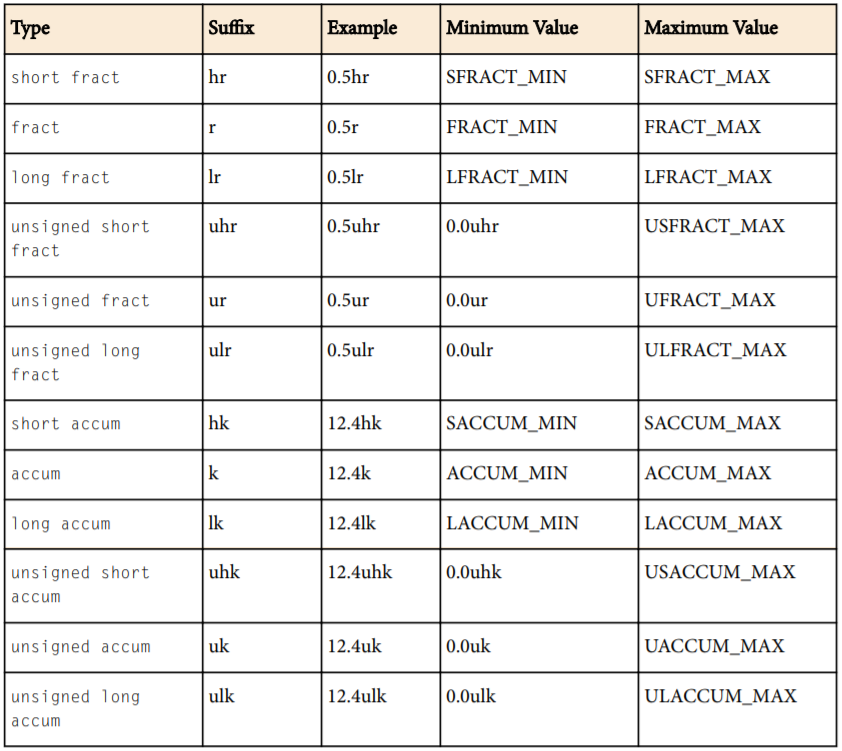
\includegraphics[width=\linewidth]{graphics/24.png}
	\caption{Suffixes and Macros, \href{http://www.analog.com/media/en/dsp-documentation/software-manuals/cces2-2-0_BlackfinCompilerAndLib_mn_rev1-6.pdf}{CrossCore Embedded Studio 2.2.0}}
	\label{fig:24}
\end{figure}

\subsubsection{Header Files}
DSP header files contain prototypes for the DSP library functions
\begin{itemize}
	\item \mintinline{c}{complex.h}
	\begin{itemize}
		\item Basic complex arithmatic functions
	\end{itemize}
	\item \mintinline{c}{cycle_count.h}
	\begin{itemize}
		\item Basic cycle counting
	\end{itemize}
	\item \mintinline{c}{cycles.h}
	\begin{itemize}
		\item Cycle counting with statistics
	\end{itemize}
	\item \mintinline{c}{filter.h}
	\begin{itemize}
		\item Filters and transformations
	\end{itemize}
	\item \mintinline{c}{math.h}
	\begin{itemize}
		\item Math functions
	\end{itemize}
	\item \mintinline{c}{matrix.h}
	\begin{itemize}
		\item Matrix functions
	\end{itemize}
	\item \mintinline{c}{stats.h}
	\begin{itemize}
		\item Statistical functions
	\end{itemize}
	\item \mintinline{c}{vector.h}
	\begin{itemize}
		\item Vector functions
	\end{itemize}
		\item \mintinline{c}{window.h}
	\begin{itemize}
		\item Window generators
	\end{itemize}
\end{itemize}

\subsection{Cycles Measurement}
\begin{itemize}
	\item Build-in macros to measure cycles
	\item Accumulates statistics
	\item Enabled by \mintinline{c}{-d DO_CYCLE_COUNTS}
\end{itemize}

\newpage \noindent \textbf{EXAMPLE cycle\_count.h}
\begin{minted}{cpp}
#include <cycle_count.h>
#include <stdio.h> 

extern int 
main(void) 
{ 
cycle_t start_count; 
cycle_t final_count; 

START_CYCLE_COUNT(start_count); 
Some_Function_Or_Code_To_Measure(); 
STOP_CYCLE_COUNT(final_count,start_count); 

PRINT_CYCLES("Number of cycles: ",final_count); 
}
\end{minted}

\noindent \textbf{EXAMPLE cycles.h}
\begin{minted}{cpp}
#include <cycles.h>
#include <stdio.h> 

extern void foo(void); 
extern void bar(void);

extern int
main(void) 
{ 
cycle_stats_t stats; 
int i; 

CYCLES_INIT(stats); 

for (i = 0; i < LIMIT; i++) { 
	CYCLES_START(stats); 
	foo();
	CYCLES_STOP(stats); 
} 
printf("Cycles used by foo\n"); 
CYCLES_PRINT(stats); 
CYCLES_RESET(stats); 


for (i = 0; i < LIMIT; i++) { 
	CYCLES_START(stats); 
	bar();
	CYCLES_STOP(stats); 
} 
printf("Cycles used by bar\n"); 
CYCLES_PRINT(stats); 
}
\end{minted}
\noindent \textbf{OUTPUT}
\begin{minted}{cpp}
Cycles used by foo 
AVG   : 25454
MIN   : 23003
MAX   : 26295 
CALLS : 16 

Cycles used by bar 
AVG   : 8727 
MIN   : 7653 
MAX   : 8912 
CALLS : 16
\end{minted}

\subsection{Complex Numbers}
\subsubsection{Datatypes}
\begin{itemize}
	\item \mintinline{cpp}{complex_float}
	\item \mintinline{cpp}{complex_double}
	\item \mintinline{cpp}{complex_fract16}
	\item \mintinline{cpp}{complex_fract32}
\end{itemize}

\subsubsection{Operations (intrinsics only)}
\begin{itemize}
	\item Absolute Value
	\item Addition
	\item Subtraction
	\item Multiply
	\item Division
	\item Conjugate
	\item Exponential
	\item Normalization
\end{itemize}

\subsection{Filter IIR, FIR- FFT, iFFT}
\subsubsection{FIR}
\begin{itemize}
	\item \mintinline{cpp}{fract16, fract32, fract, long fract}
\end{itemize}

\begin{minted}{cpp}
#include <filter.h>

fir_init(state, coeffs, delay, NUM_COEFFS, 0);
fir_fr32(input, output, NUM_SAMPLES, &state);
\end{minted}

\subsubsection{IIR}
\begin{itemize}
	\item \mintinline{cpp}{fract16, fract32, fract, long fract}
\end{itemize}

\begin{minted}{cpp}
#include <filter.h>
                  
iir_init (filter_state,coeffs,delay,NUM_STAGES); 
iir_fr16 (signal,output,NUM_SAMPLES,&filter_state);
\end{minted}

\subsubsection{FFT}
\begin{itemize}
	\item Discrete Fourier Transformation
	\begin{itemize}
		\item Transform from time to frequency domain
		\begin{itemize}
			\item Sum of products with time-domain sequence of sine and a cosine wave
		\end{itemize}
		\item Digital signal $x(n)$, a finite-duration sequence of length $N$
	\end{itemize}
\end{itemize}

\begin{equation}
X(k)=\sum_{n=0}^{N-1}x(n)e^{-j\frac{2\pi}{N}kn}
\end{equation}

\begin{itemize}
	\item Defining a Twiddle factor $W_N$
\end{itemize}

\begin{equation}
W_N=e^{-j\frac{2\pi kn}{N}}=\cos\left(\dfrac{2\pi kn}{N}\right)-j\sin\left(\dfrac{2\pi kn}{N}\right)
\end{equation}

\begin{itemize}
	\item DFT defined by a Twiddle factor
\end{itemize}

\begin{equation}
X(k)=\sum_{n=0}^{N-1}x(n)W_N^{kn}\;,\,k=0,1,...,N-1
\end{equation}

\begin{itemize}
	\item ݇$k$ is the frequency index
	\item Frequency spacing is ݂$\frac{f_s}{N}$
	\item ܺ$X(k)$ are complex values
	\begin{itemize}
		\item Magnitude and phase components
	\end{itemize} 
\end{itemize}

\begin{equation}
X(k)=Re[X(k)]+jIm[X(k)]=|X(k)|e^{j\phi(k)}
\end{equation}

\begin{itemize}
	\item FFT is a fast computational version of DFT
	\begin{itemize}
		\item \textit{N}-point DFT radix-2, here \textit{N} must be a power of 2 
	\end{itemize}
\end{itemize}

\begin{equation}
\dfrac{FFT}{DFT}=\dfrac{\log_2N}{2N}
\end{equation}

\begin{itemize}
	\item Twiddle table
\end{itemize}

\begin{minted}{cpp}
twidfftrad2_fr16(m_twiddle_table,N_FFT);
\end{minted}

\begin{itemize}
	\item FFT and magnitude
\end{itemize}

\begin{minted}{cpp}
rfft_fr16(input,m_fft_output,m_twiddle_table,1,N_FFT,&block_exponent,2);

fft_magnitude_fr16(m_fft_output,m_real_magnitude,N_FFT,block_exponent,1);
\end{minted}


